\documentclass[12pt,letter]{article}
\usepackage[utf8]{inputenc}
\usepackage{graphicx}
\usepackage{amsmath}
\usepackage{amsfonts}
\usepackage{amssymb}
\usepackage[toc,page]{appendix}
\author{Martin Ambrozic}
\title{Notes on Neural Net Q-value Estimator for Volleyball}
\date{}

\newcommand{\bb}[1]{\mathbf{#1}}

\def\Xint#1{\mathchoice
	{\XXint\displaystyle\textstyle{#1}}%
	{\XXint\textstyle\scriptstyle{#1}}%
	{\XXint\scriptstyle\scriptscriptstyle{#1}}%
	{\XXint\scriptscriptstyle\scriptscriptstyle{#1}}%
	\!\int}
\def\XXint#1#2#3{{\setbox0=\hbox{$#1{#2#3}{\int}$ }
		\vcenter{\hbox{$#2#3$ }}\kern-.6\wd0}}
\def\ddashint{\Xint=}
\def\dashint{\Xint-}

\begin{document}
	
	\maketitle
	
	\subsection*{Neural Network Architecture}
	
	The neural network architecture is based on \cite{liu2018deep}. The layers are:
	\begin{itemize}
		\item First layer containing 256 LSTM nodes for sequence processing,
		\item Hidden dense layer of 1000 nodes with RelU activation,
		\item Output layer.
	\end{itemize}
	The input sequence contains vectors of the current state-action pair and a history of up to 9 previous state-action pairs in the same rally.\\\\
	The network outputs a single number, which is the estimated expected reward value of the given state sequence. This differs from the implementation in \cite{liu2018deep}, where separate values are output for 'home score', 'away score' and 'no score' events. Because of the nature of scoring in volleyball, every rally ends with one of the two teams scoring and only a single number is sufficient to describe all outcomes.

	\subsection*{Convergence}
	
	We define an iteration as one full training pass through the entire dataset. Our convergence measure is the mean absolute difference between Q value estimates of consecutive iterations, i.e. for iteration $i$ we have:
	$$e_i = \frac{1}{n}\|Q_i - Q_{i-1}\|_1,$$
	where $Q_i$ is the i-th iteration vector of Q value estimates for the entire dataset and $n$ is the number of entries in the dataset. Figure \ref{fig:nn_convergence} shows a plot of $e_i$ values per iteration for a sample training run. We stop training when $e_i < 0.0005$ \\\\
	
	\begin{figure}
		\centering
		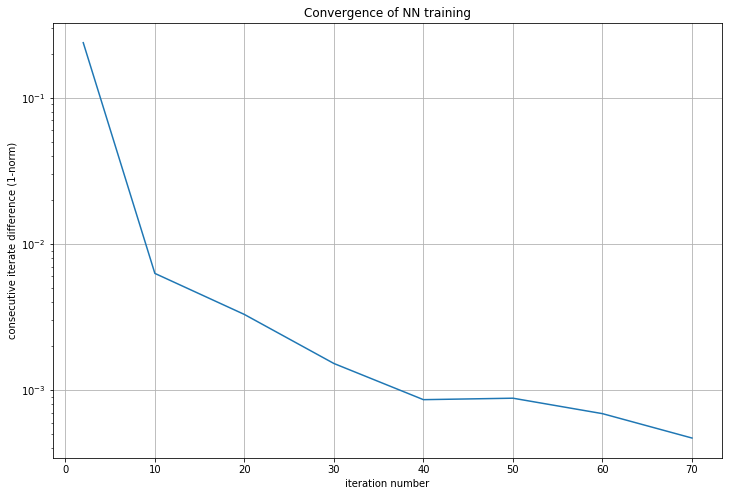
\includegraphics[scale=0.5]{images/nn_convergence.png}
		\caption{Convergence of neural network training.}
		\label{fig:nn_convergence}
	\end{figure}
	
	\subsection*{Comparison of Q Values to Decision Tree}
	
	Q values learned by the neural network and those learned by a decision tree classifier are close, but not identical.\\\\
	The mean absolute Q value difference between the two methods over the entire dataset is 0.065. Instances of the Q value estimates being very far apart are rare, eg. there are 244 occurrences where $|Q_{tree}-Q_{NN}| > 1$. On that particular subset, the neural net performs substantially better, achieving 85\% accuracy as a classifier as opposed to merely 15\% accuracy of the decision tree. In short, wherever Q values by the NN deviate far from those of the tree, it is usually the neural net that is correct.\\\\
	Table \ref{tab:action_outcomes} shows a breakdown of average Q values for the Home Attack action, grouped by the action's outcome. Outcomes '=', '/' and '\#' constitute the rally ending, so we expect the Q value to be 1 or -1 in those instances. We note that the values are qualitatively similar, but not quite identical.
	
	\begin{table}[]
		\centering
		\begin{tabular}{lll}
			\textbf{Attack Outcome} & \textbf{Q by Neural Network} & \textbf{Q by Decision Tree} \\ \hline
			=                        & -1.000                       & -0.932                      \\
			/                        & -0.988                       & -0.920                      \\
			-                        & -0.060                       & -0.069                      \\
			!                        & 0.111                        & 0.092                       \\
			+                        & 0.373                        & 0.288                       \\
			\#                       & 1.008                        & 0.986                      
		\end{tabular}
		\caption{Average Q values by attack action outcome - comparison between neural network and decision tree estimator.}
		\label{tab:action_outcomes}
	\end{table}
	
	\newpage
	
	\bibliography{references}
	\bibliographystyle{ieeetr}

\end{document}